\documentclass[a4paper,twoside,12pt,fleqn]{scrartcl}
\usepackage[margin=2.5cm]{geometry}
%\usepackage{fancyref}
%\usepackage{graphicx}
%\usepackage{float}
%\usepackage{tabularx}
%\usepackage{booktabs,array}
%\usepackage{caption}
\usepackage{subcaption}
\usepackage{amsmath}
\usepackage{amsthm}
\usepackage{amssymb}
\usepackage{mathtools} % for multlined enviornment
%\usepackage{amsfonts}
%\usepackage{enumitem}
\usepackage[hyphens]{url}
\geometry{a4paper}
\usepackage{amssymb}%---allows \mathbb{R/Z/etc.} (numbers sets)
\usepackage{scrextend} %for eddmargin environment
\usepackage{caption}
\usepackage{titlesec}


%%%%[for python code] %%%%%%
\usepackage{listings}
\usepackage{color}

\definecolor{dkgreen}{rgb}{0,0.6,0}
\definecolor{gray}{rgb}{0.5,0.5,0.5}
\definecolor{mauve}{rgb}{0.58,0,0.82}

\lstset{frame=tb,
  language=Python,
  aboveskip=3mm,
  belowskip=3mm,
  showstringspaces=false,
  columns=flexible,
  basicstyle={\small\ttfamily},
  numbers=none,
  numberstyle=\tiny\color{gray},
  keywordstyle=\color{blue},
  commentstyle=\color{dkgreen},
  stringstyle=\color{mauve},
  breaklines=true,
  breakatwhitespace=true,
  tabsize=3
}

%\titlelabel{\thetitle\quad}


\renewcommand{\vec}[1]{\mathbf{#1}}
\newcommand{\parder}[2]{\frac{\partial{#1}}{\partial{#2}}}

\newcommand{\sectionbreak}{\clearpage}

\newcommand{\lagrangian}[1]{\mathcal{L}(\vec{#1})}
\newcommand{\vecprod}[2]{\vec{#1}^T{\vec{#2}}}
\newcommand{\expwx}{\exp(\vecprod{w}{x}_i)}
\newcommand{\sumn}[2]{\sum_{#1 = 1}^{#2}}
\newcommand{\sums}[1]{\sum_{s'\in\mathbb{S}} P(s' | \bar{s},#1)}

\renewcommand{\thesubsection}{\thesection.\alph{subsection}}

\usepackage{etoolbox}
\patchcmd{\thebibliography}{\subsubection*}{}{}{}

\DeclareMathOperator*{\argmax}{arg\,max}

\begin{document}
\title{Reinforcement Learning\\Homework Sheet 3}
\subtitle{Lawrence Kurowski 2019280743}
\date{12 May 2020}
\maketitle

\section{PPO}\label{PPO}

We construct PPO using Tensorflow / Keras library.

The PPO model has 2 networks: actor and critic network. Actor network is the policy network and the loss function is the PPO loss, calculated as (pseudo-code):
\begin{lstlisting}
ratio = exp( log(newpolicy_pi)  - log(oldpolicy_pi) )

# following the formulas from the PPO paper
val_1 = ratio * advantages
val_2 = K.clip(ratio, min_value=1 - clipping_val, max_value=1 + clipping_val) * advantages

actor_loss = - mean(K.minimum(val_1, val_2))
\end{lstlisting}

Here we calculate advantages using the recursive formula for GAE (pseudo-code):
\begin{lstlisting}
delta = rewards[i] + gamma * values[i + 1] * masks[i] - values[i]
gae = delta + gamma * lmbda * masks[i] * gae
\end{lstlisting}

We train the PPO over 100 episodes, and let it play until ``done'' and for max. 100 steps inside each episode.

In each episode, after experienced is collected, the actor and critic nets are updated and environment reset.

Early-stopping is introduced when the system starts scoring positive reward (goal).

We show the value (critic) and policy (actor) loss plot as function of training episodes in figure \ref{fig_ppo_losses} (a) and (b), respectively.

After training is completed, we run the game for 100 episodes, each time allowing for a max. of 100 ``moves'' before terminating the game. We record rewards and plot in figure \ref{fig_ppo_rewards} (a). The cumulative rewards over 100 testing steps is shows in figure \ref{fig_ppo_rewards} (b). 

\begin{center}
\begin{tabular}{lclc}
(a) &
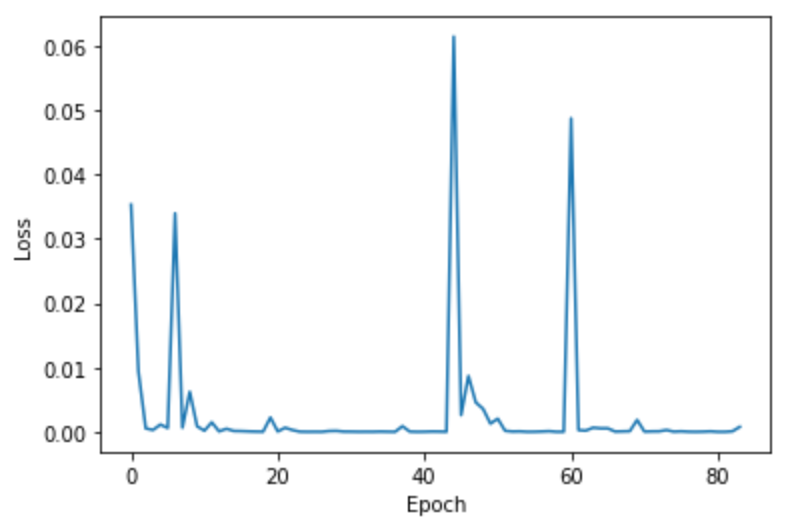
\includegraphics[width=5cm]{fig_ppo_loss_critic.jpg}
& (b)
&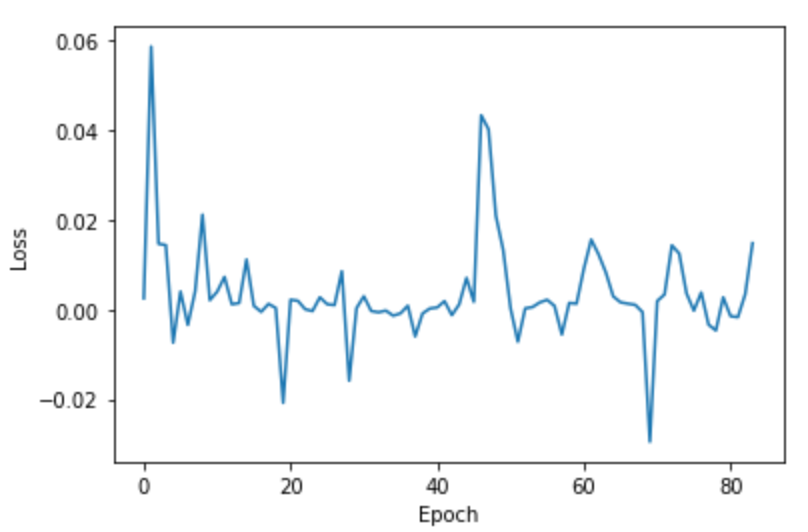
\includegraphics[width=5cm]{fig_ppo_loss_actor.jpg}
\end{tabular}
\captionof{figure}{(a) critic (value) and (b) actor (policy) PPO model training loss.}
\label{fig_ppo_losses}
\end{center}

\begin{center}
\begin{tabular}{lclc}
(a) &
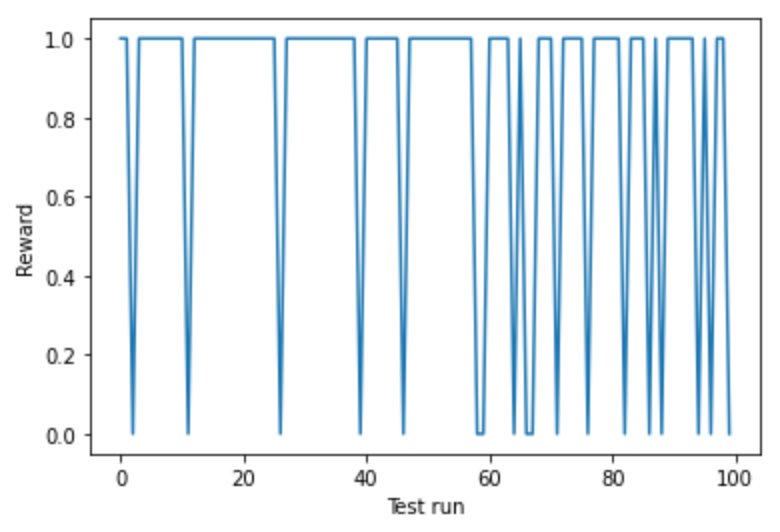
\includegraphics[width=5cm]{fig_ppo_reward.jpg}
& (b)
&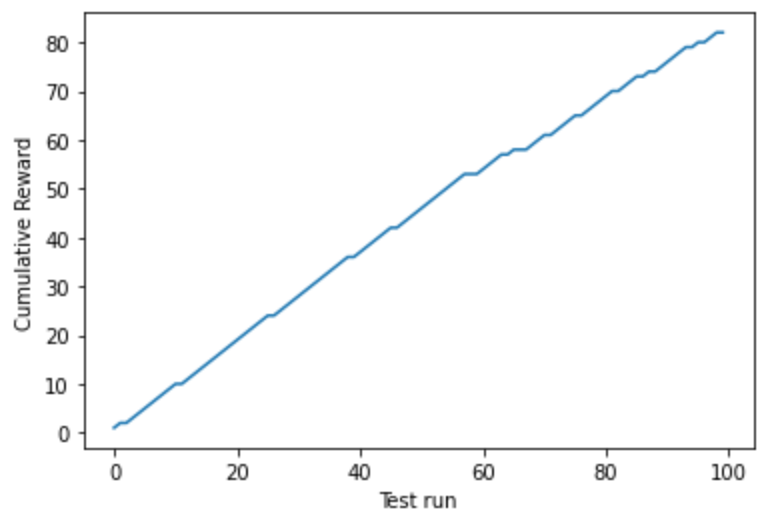
\includegraphics[width=5cm]{fig_ppo_reward_cum.jpg}
\end{tabular}
\captionof{figure}{Rewards for 100 test steps of the PPO model. (a) shows the rewards, while (b) is the cumulative reward.}
\label{fig_ppo_rewards}
\end{center}
\section{DDPG}\label{DDPG}

We construct DDPG using Tensorflow / Keras library, using similar code structure / ideas to PPO in section \ref{PPO}.

The DDPG model has 2 networks: actor and critic network, as well as 2 target networks actor target and critic target. 

We also use the target networks to optimize the model. In particular, at each step we first update the prediction and then minimize according to the MSE loss (pseudo-code):
\begin{lstlisting}
# generate critic preds
Qvals = critic.predict([next_state, action])
# generate actor-derived predictions for next action
next_actions = actor_target.predict([next_state])
# Q updates
next_Q = critic_target.predict([np.array(next_state_batch) , np.array(next_actions)])
Qprime = (reward_batch) + gamma * next_Q

# MSE loss
loss = mean_squared_error(Qprime, Qvals)
\end{lstlisting}

Here the ``batch'' refers to samples from the ``replay buffer'', or in other words from the already played out scenarios. 

While actor and critic networks are trained with back-propagation, the target networks are updated at each step according to (pseudo-code):
\begin{lstlisting}
params = tau * actor_model_params + (1-tau) * target_actor_model_params
params = tau * critic_model_params + (1-tau) * target_critic_model_params
\end{lstlisting}

We train the DDPG over 100 episodes, and let it play until ``done'' and for max. 1000 steps inside each episode.

In each episode, after experienced is collected, the actor and critic nets are updated and environment reset.

Early-stopping is introduced when the system starts scoring positive reward (goal).

Unfortunately, our model did not yield satisfying results despite training for a long time, and eventually we ran out of time before the submission deadline. We hope that the attached file (``DDPG'') explains our reasoning in how we designed the code.
%\section{}\label{question3}

Let $\tilde{V}$ be some value function, $V_g$ be the greedy value function and $V^*$ be the optimal value function. Let $\mathbb{S}$ and $\mathbb{A}$ be the state and action spaces, respectively. Let $\epsilon>0$.

For value function $V$ and $s\in \mathbb{S}$ define $L_V(s) = |V(s) - V^*(s)|$ which is the value loss if we choose a sub-optimal policy.

\subparagraph{CLAIM} $|\tilde{V} - V^*|<\epsilon \Rightarrow <\frac{2\epsilon \gamma}{1-\gamma}$.

\subparagraph{PROOF}

Let $\bar{s} = \argmax_{s\in\mathbb{S}} L_{\tilde{V}}(\bar{s})$. This exists by the assumption in CLAIM.

Let $a\mathbb{A}$ be the optimal choice $\pi^*(\bar{s}) = a$ and $b$ be the greedy choice $\pi_g(\bar{s})=b$.

Because $b$ is chosen with greedy policy, it has to be at least as good as $a$:
\begin{equation}
\tilde{V}(s) = R(\bar{s},a)+\gamma \sums{a} \tilde{V} (s') \leq R(\bar{s},b) + \sums{b} \tilde{V}(s')
\label{eq1}
\end{equation}
By assumed property, $ V^*(s) - \epsilon< \tilde{V}(s) <V^*(s) + \epsilon, \forall s\in\mathbb{S}$, hence \eqref{eq1} gives
\begin{equation*}
R(\bar{s},a)+\gamma \gamma \sums{a} \left(V^* (s')-\epsilon\right) \leq R(\bar{s},b) + \gamma \sums{b} \left(V^*(s')+\epsilon \right)
\label{eq2}
\end{equation*}

hence
\begin{equation}
R(\bar{s},a)-R(\bar{s},b) \leq 2\gamma \epsilon + \gamma \sum_{s'\in\mathbb{S}}\left( P(s' | \bar{s},b) V^*(s') - P(s' | \bar{s}, a) V^*(s')\right)
\label{eq3}
\end{equation}

Because $\bar{s}$ was chosen so that it maximizes $L_V(s)$ for an arbitrary value function $V$, in particular it maximizes the loss for the greedy policy value function $L_{V_g}$, hence, using the fact that $g$ is the greedy policy choice, as well as \eqref{eq3} we have
\begin{align*}
L_{V_g}(\bar{s}) = & V^*(\bar{s}) - V_g(\bar{s}) \\
= & R(\bar{s},a)-R(\bar{s},b) + \gamma \sum_{s'\in\mathbb{S}}\left( P(s' | \bar{s},a) V^*(s') - P(s' | \bar{s}, b) V_g^*(s')\right) \\
\leq & 2\epsilon \gamma + \gamma \sum_{s'\in\mathbb{S}}\left( P(s' | \bar{s},b) V^*(s') - P(s' | \bar{s},a) V^*(s') + P(s' | \bar{s}, a) V^*(s') - P(s' | \bar{s},b) V_g^*(s')\right)\\
&= 2\epsilon \gamma + \gamma \sum_{s'\in\mathbb{S}}\left( P(s' | \bar{s},b) V^*(s') - P(s' | \bar{s},b) V_g(s')\right)\\
&=2\epsilon \gamma + \gamma \sums{b} L_{V_g}(s')\\
&\leq 2\epsilon\gamma + \gamma \sums{b} L_{V_g}(\bar{s})
\end{align*}
rearranging we get that for every $s\in\mathbb{S}$
\begin{equation*}
L_{V_g}(s) = \leq L_{V_g}(\bar{s}) \leq \frac{2\epsilon\gamma}{1-\gamma}
%\label{eq2}
\end{equation*}
Q.E.D.


%\input{AccuracyLoss}

\end{document}